
\chapter{Thomas's Tangles}


Computing, and Computational Thinking in general,  is not just about programming and using a computer (though using computers and  programming are vitally important to Computing); but it is also about many other things including problem-solving, being creative and working collaboratively.

This chapter (and activity) are about linking these computational thinking ideas to produce visual art, by applying computing principles. 

Did you know that some artists such Sol Le Witt \url{https://en.wikipedia.org/wiki/Sol_LeWitt} did not physically produce all the work credited to themselves. In some cases the actual physical work was made by others following the artist's exact written instructions - in other words an algorithm. This meant that the work can be shown in a number of places at the same time.

\section{Tools we can use}

In this activity we are are going to write out a set of clear instructions(we hope) that mean another person can follow them and carry out actions exactly (that is a challenge) as we planned. Our \textbf{three tools} are going to be 
\begin{itemize}
    \item sequences
    \item repetition/loops
    \item tests
\end{itemize}


Before we start a few things to remember, that I find useful when doing these types of activities:
\begin{itemize}
    \item Computers are not intelligent; we have to tell it literally what to do.
    \item You're the boss, you tell the machine what to do not the other way around.
    \item You are not writing the instructions for you do to the activity but for someone else. They must be able to do follow these without coming back to you and asking "What did you mean here?"
    \item There is not one answer to these activity, your solution and another group's can both be right.  
    \item We need test and find things we have missed - it is not personal.
\end{itemize}

So let's look at our three tools using an example of opening a bottle.

A sequence of instructions
\begin{lstlisting}
Find the lid of a bottle
Turn lid of the bottle until lid comes off
\end{lstlisting}

A loop to repeat a sequence until something we define happens or even to continue forever. So our instruction "Turn lid of the bottle until lid comes off" might be changed to break it down further to produce a certain sequence of instructions to be repeated. I am going use indenting to show what is inside the loop (the bit that repeats).
\begin{lstlisting}
hold the bottle
Repeat until lid comes off
   turn the lid 45 degrees anti-clockwise
   release lid hand 
   move lid back starting position
   check does the lid come off?
\end{lstlisting}

Our last tool is a test (conditional statement) where we can change what happens based on the outcome of the test. Again I i am going to use indenting to show what belongs togther. In the previous 'code' we had a line saying "check does the lid come off?" which was two outcome if the lid does come off or it doesn't, This sounds like a test

\begin{lstlisting}
if check does the lid come off == yes
   pull the lid vertical 10 cm
   stop the algorithm
\end{lstlisting}

So lets put all of these together
\begin{lstlisting}
Find the lid of a bottle
hold the bottle
Repeat until lid comes off
   turn the lid 45 degrees anti-clockwise
   release lid hand 
   move lid back starting position
   if check does the lid come off == yes
     pull the lid vertical 10 cm
     stop the algorithm
\end{lstlisting}

So know we have a starting point for a routine/algorithm for opening a bottle. 

\section{Activity - Make your own Art game}
This activity is about using computing ideas to build a paper-based game. Aim is to create pictures by developing and then following a set of instructions (Algorithms). We are going to use the three tools to make the games. 

Goal 1: At the end of the session you have produce a paper-based game's instructions that use dice, pens and paper to produce random drawings (see Figure 5.1). The instructions will probably look a bit like the bottle opening routine 

Goal 2: You have tested some one else's game and constructively feedback to the developers, ideas, improvements, etc. Testing is an important part of Computing.


Task: \textbf{Develop in groups of 2-3 people, a paper-based game's instructions that use dice, pens and paper to produce random drawings. It must use the 'Three Tools', dice, pens and paper; BUT how you use them is up to you. Your instructions will be in sentences so the user can understand exactly what you mean. Your group must test another group's game and provide constructive help.} 


You have two dice, some pens and paper.

First 20 minutes
Working in groups of 2-3 people, develop your games and produce the instructions.

Remaining Time
Swap your game with another group and each try their game. Pass back constructive feedback to the other group. Some suggestions to possibly ask yourself when testing.
\begin{itemize}
    \item Could a particular instruction be viewed as meaning something else?
    \item Is there something the developer's could add to improve the game in your opinion?
\end{itemize}

Don't panic: In case of emergency in the next section there is an example, please build your own first.


\section{Thomas Tangles}
This is an example of the type of solution that could be built. Aim for your's to be better than this one.

Using crayons, pencils or pens, we are going to follow an algorithm to create a random drawing. This could be done in pairs and you will need squared paper. 

Person A: Rolls the dice and reads out the instructions - their role is to roll the dice, interpret the algorithm and tell the 'robot' what to do.

Person B: Is the ‘robot carrying out the instructions'. The lines are solid blocks of colour so move four squares does also mean colour in the squares between the start and finish in the direction of movement.

\begin{figure}
    \centering
    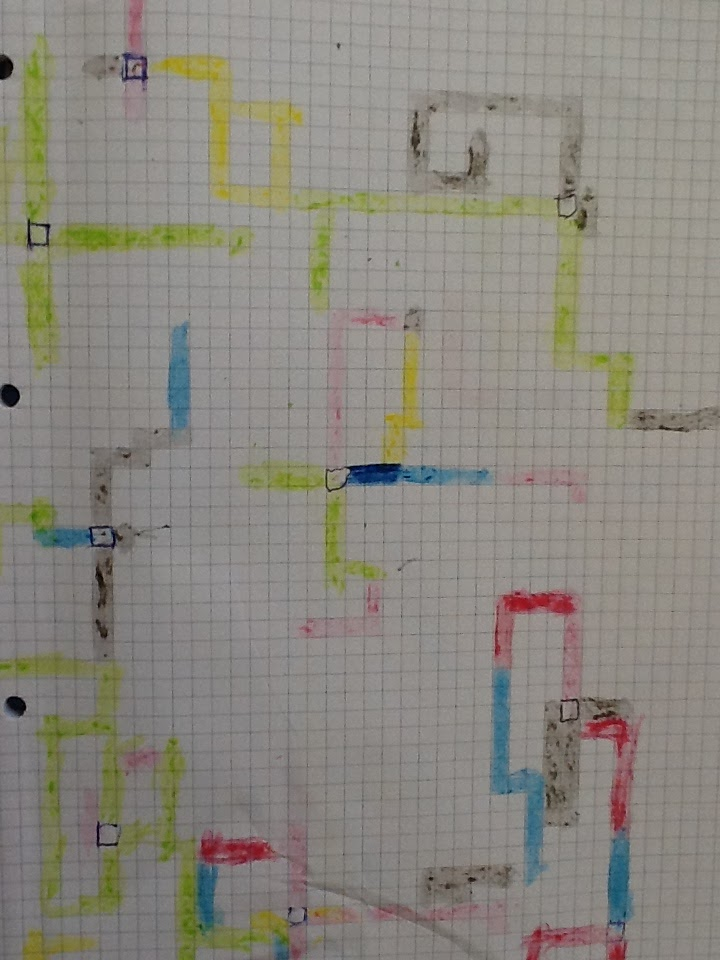
\includegraphics[width=10cm]{chapters/chapterCT1/figures/tt1.JPG}
    \caption{Thomas' Tangles}
    \label{fig:ThomasTangles1}
\end{figure}

When a new central square is needed the roles of A and B swap (so A is the ‘robot’ and B rolls the dice and reads out the instruction). The roles keep swapping.

\begin{lstlisting}
Start from a random square – call it the centre square
Repeat until end of game
If die roll = 1
  Roll die for number of moves
 move die roll number of steps up the page
If die roll = 2
  Roll die for number of moves
  move die roll number of steps down the page
If die roll = 3
  Roll die for number of moves
  move die roll number of steps to the left 
If die roll = 4
  Roll die for number of moves
  move die roll number of steps to the right
If die roll = 5
  Roll die
  If die = 1 change colour to Red
  If die = 2 change colour to Blue
      If die = 3 change colour to Black
  If die = 4 change colour to Green
  If die = 5 change colour to Orange
  If die = 6 change colour to Yellow
If die roll = 6
           Roll die
           Return to current centre square
           If the second die roll=6
                   randomly select new centre square
                   if block is off the page
                      randomly select new centre square
\end{lstlisting}

The Scratch version can be here \url{https://scratch.mit.edu/projects/135816631/} if you wish to see the code.

